\documentclass[10pt,a4paper]{article}
\usepackage[utf8]{inputenc}
\usepackage[czech]{babel}
\usepackage[T1]{fontenc}
\usepackage{amsmath}
\usepackage{amsfonts}
\usepackage{amssymb}
\usepackage{graphicx}
\usepackage{float}

\author{Martin Žid}
\title{Řešení problému vážené splnitelnosti booleovské formule pokročilou iterativní metodou}
\date{}
\begin{document}

\maketitle

\section{Zadání}
Problém vážené splnitelnosti booleovské formule řešte některou z pokročilých lokálních heuristik (simulované ochlazování, genetické algoritmy, tabu prohledávání). Volby konkrétních parametrů heuristiky a jejích detailů (operace nad stavovým prostorem, kritérium ukončení, atd. atd.) proveďte sami, tyto volby pokud možno zdůvodněte a ověřte experimentálním vyhodnocením. Hodnotí se především postup při aplikaci heuristiky, tj. postup a experimenty, jakým jste dospěli k výsledné podobě (parametry, konkrétní operátory apod.). Například, pokud máte v řešení nějaké hodně neortodoxní prvky a pokud máte jejich výhodnost experimentálně doloženou, těžko mohou vzniknout námitky. Méně významné jsou konkrétní dosažené výsledky.

Tato práce by měla sloužit jako ověření Vašich schopností používat zvolenou pokročilou iterativní metodu. Ideálním výstupem by měl být algoritmus schopný řešit co nejširší spektrum instancí s rozumnou chybou. To neznamená, že pokud se Vám některé instance \uv{nepovedou}, je vše špatně. Důležité je, abychom viděli, že jste se aspoň snažili.

 \subsection{Problém}
Je dána booleovská formule $F$ proměnných $X=(x_1, x_2, ..., x_n)$ v konjunktivní normální formě (tj. součin součtů). Dále jsou dány celočíselné kladné váhy $W=(w_1, w_2,... , w_n)$. Najděte ohodnocení $Y=(y_1, y_2, … , y_n)$ proměnných $x_1, x_2, … , x_n$ tak, aby $F(Y)=1$ a součet vah proměnných, které jsou ohodnoceny jedničkou, byl maximální.
 
Je přípustné se omezit na formule, v nichž má každá klauzule právě 3 literály (problém 3 SAT).

\section{Rozbor možných variant řešení}
V této úloze jsme měli možnost výběru jedné ze tří pokročilých iterativních technik.
Algoritmy k výběru:
\begin{itemize}
 \item simulované ochlazování,
 \item genetické algoritmy,
 \item tabu search.
\end{itemize}
Pro řešení této úlohy jsem si zvolil metodu simulovaného ochlazování, se kterou jsem již implementoval problém batohu v minulé úloze.

\section{Rámcový popis postupu řešení}
V první části jsem implementoval generátor vah, který přijímá instanci problému \uv{DIMACS CNF} (z http://www.cs.ubc.ca/\~hoos/SATLIB/benchm.html). Pro daný problém vygeneruje váhy v rozsahu 0-100 a uloží tento rozšířený problém do nového souboru.

Následně byl vytvořen program pro řešení výše popsaných problémů a to pomocí metody simulovaného ochlazování. Při implementaci jsem za zajímal o~vhodnou formu cenové funkce (popsáno v další kapitole). Nakonec probíhalo měření a to jak vhodné nastavení cenové funkce, tak i závislost výpočtu na jednotlivých parametrech algoritmu. Při měření byl měněn vždy pouze jeden parametr a ostatní byly zafixovány.

\section{Popis kostry algoritmu}
Algoritmus má nastavitelné čtyři parametry: počáteční teplotu, koncovou teplotu, $equilibrium$ a koeficient ochlazování.

Na začátku je vybrán počáteční stav, což je implementováno jako nastavení všech proměnných na 0 ($false$) a teplota je rovna počáteční teplotě. Následný výpočet probíhá ve dvou cyklech. Počet iterací vnějšího cyklu udává funkce $frozen$ a vnitřního cyklu funkce $equilibrium$. Funkce $frozen$ vrací $true$, pokud teplota dosáhla hodnoty koncové teploty. Funkce $equilibrium$ vrací $true$, pokud je počet iterací na dané teplotě menší než $n * equilibrium$.

Ve vnitřním cyklu je volána funkce $try$. Funkce $try$ náhodně zvolí (změnou jednoho bitu vektoru konfigurace) souseda aktuálního stavu. Pokud je tento soused lepší než daný stav, pak je vrácen. Pokud není, je vrácen pouze pokud $ x < e^{\frac{-\delta}{teplota}}$. Kde $x$ je náhodné číslo z intervalu 0, 1 a $\delta$ je rozdíl vah nového a aktuálního stavu. Ve všech ostatních případech je vrácen původní stav.

Ve vnitřním cyklu je ještě testováno zda nemá aktuální stav vyšší váhu než nejlepší naleznou. Pokud ano a zároveň je tento stav \uv{SAT} ($F(Y)=1$), pak je daný stav uložen jako nejlepší.

Po doběhnutí vnitřního cyklu $equilibria$ je volá funkce $cool$, která vynásobí teplotu koeficientem ochlazování. Tento koeficient je v rozmezí 0,8 až 0,99 (teplotu tedy zmenší).

Algoritmus není omezený na 3SAT.

\subsection{Rozšíření oproti problému batohu}
U problému batohu bylo velice jednoduché najít řešení (již např. prázdný batoh), a tudíž i při změně konfigurace jsme měli velkou šanci pro nalezení konfigurace, která je řešením. Toto však neplatí u problému vážené splnitelnosti booleovské formule, proto bylo nutné (pro lepší hledání řešení) zvýhodňovat řešení, co mají větší počet splněných klauzulí. Toto povede až k nalezení stavu, který má splněné všechny klauzule, tedy \uv{SAT}.

První návrh tohoto řešení bylo ve funkci $better$ vybírat lepší stav problému nejprve pouze podle počtu splněných klauzulí a ignorovat jejich váhu. Až pokud měly stavy stejný počet splněných klauzulí, tak porovnat jejich váhu. Toto řešení však nebylo ideální, protože v druhé části funkce $try$ se na výpočet $\delta$ používá funkce $weight$ a funkce $better$ se zde neobjevuje.

Druhé, již použité, řešení bylo upravení funkce $weight$, která se používá i~ve funkci $better$. Zvýhodnění bylo závislé na parametru $coef$. Pokud stav nebyl \uv{SAT}, výstupem byl výsledek vzorce $weight*clausesTrue^{coef}$, kde $weight$ je skutečná váha stavu a $clausesTrue$ je počet splněných klauzulí. Na druhou stranu pokud stav splňoval $F(Y)=1$, byla jeho váha vynásobena parametrem $coef$. Volba hodnoty $coef$ musela být otestována, protože při příliš malé hodnotě bude menší šance na najití stavu, který je řešením. A pří nastavení hodnoty $coef$ na přehnaně vysokou, bude hrozit uvíznutí v lokálních optimech, protože řešení \uv{SAT} bude příliš zvýhodněno a nebude muset dojít k jeho opuštění.

\section{Měření}
Základní nastavení algoritmu bylo: počáteční teplota = 500, koeficient ochlazování = 0,93, teplota tuhnutí = 1, $equilibrium$ = 400. Základní měření probíhalo na souborech 1-20 uf20-91 (všechny splnitelné). 

Ještě před započetím měření byly odhadovány nejlepší řešení daných problémů. Tento odhad byl prováděn opakovaným spouštěním všech dvaceti souborů pro velké množství iterací algoritmu (okolo 1,5 milionu). Nejlepší nalezené hodnoty byly zaznamenány a následně používány v měření.

\subsection{Měření optimálního nastavení zvýhodňujícího koeficientu}

\begin{table}[H]
\centering
  \begin{tabular}{ |l|l|l|}
  \hline
  Zvýhodňující koeficient & Počet nejlepších řešení & Počet nalezených řešení (SAT)\\
  \hline
    1  & 2 & 5  \\
    2  & 6 & 7  \\
    4  & 8 & 8  \\
    6  & 9 & 9  \\
    8  & 8 & 10 \\
    12 & 7 & 10 \\  
  \hline
  \end{tabular}
  \caption{Závislost vyřešených problémů a nalezených nejlepších řešení na koeficientu zvýhodnění}
\end{table}

Toto měření probíhalo pro deset souborů. Tedy hodnoty jsou vždy $x$ z 10. Měření potvrdilo předpoklad, neschopnost nalezení \uv{SAT} stavů při nízkém koeficientu a možnost uvíznutí v lokálních optimech při příliš vysokém koeficientu. Jako ideální hodnota nastavení koeficientu bylo zvoleno 6.

\begin{figure}[H]\centering
 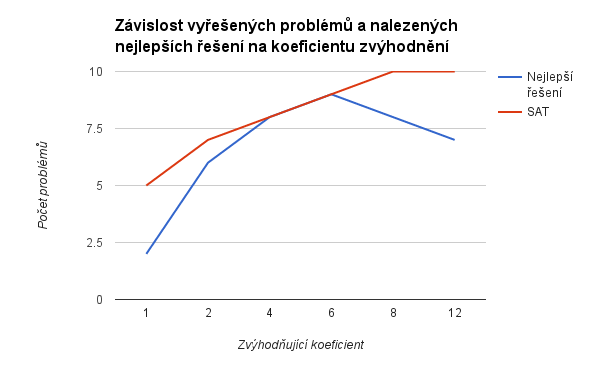
\includegraphics[width=0.99\textwidth]{1}
\end{figure}

\subsection{Závislost výpočtu na jednotlivých parametrech algoritmu}
Při měření byl měněn vždy jeden parametr a všechny ostatní byly zafixovány. Měření probíhalo s již nastavených koeficientem zvýhodnění na hodnotu 6. A bylo měřeno vždy 20 souborů. Tedy hodnoty \uv{Počet nejlepších řešení} a \uv{Počet nalezených řešení (SAT)} jsou vždy $x$ z 20.

\begin{table}[H]
\centering
  \begin{tabular}{ |l|l|l|l|}
  \hline
  Počáteční teplota & \# nalezených řešení & \# nejlepších řešení & Iterace\\
  \hline
    50   & 16 & 14 & 216000 \\
    100  & 17 & 15 & 256000 \\
    200  & 18 & 16 & 296000 \\
    500  & 19 & 17 & 344000 \\
    1000 & 19 & 17 & 384000 \\ 
  \hline
  \end{tabular}
  \caption{Závislost vyřešených problémů, nalezených nejlepších řešení a iterací na počáteční teplotě}
\end{table}

Na naměřených datech je možné vidět ideální nastavení počáteční teploty v rozmezí 400-600.

\begin{figure}[H]\centering
 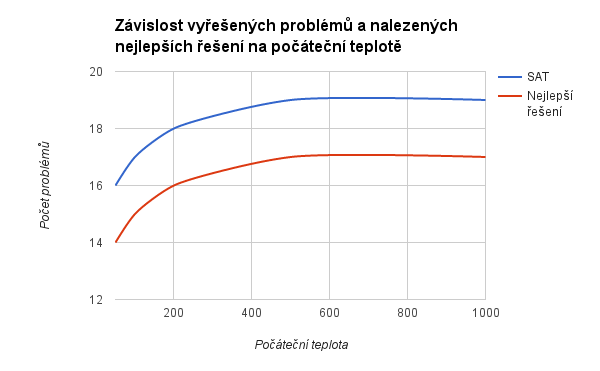
\includegraphics[width=0.99\textwidth]{2}
\end{figure}

\begin{figure}[H]\centering
 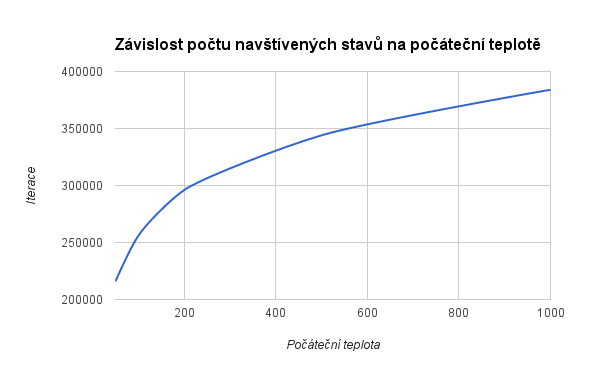
\includegraphics[width=0.99\textwidth]{3}
\end{figure}

\begin{table}[H]
\centering
  \begin{tabular}{ |l|l|l|l|}
  \hline
  Koef. ochlazování & \# nalezených řešení & \# nejlepších řešení & Iterace\\
  \hline
    0,8  & 16 & 14 & 112000 \\
    0,85 & 16 & 14 & 156000 \\
    0,90 & 17 & 16 & 236000 \\
    0,93 & 19 & 17 & 344000 \\
    0,96 & 19 & 17 & 612000 \\
  \hline
  \end{tabular}
  \caption{Závislost vyřešených problémů, nalezených nejlepších řešení a iterací na koeficientu ochlazování}
\end{table}


\begin{figure}[H]\centering
 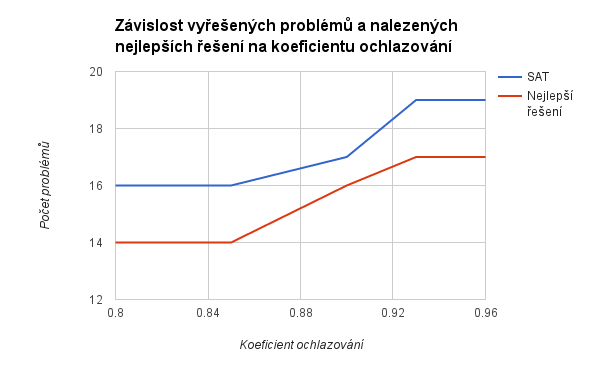
\includegraphics[width=0.99\textwidth]{4}
\end{figure}

\begin{figure}[H]\centering
 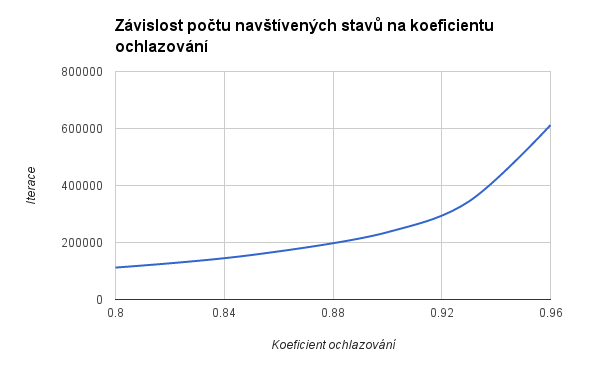
\includegraphics[width=0.99\textwidth]{5}
\end{figure}

Vhodné nastavení koeficientu ochlazování je možné odhadovat okolo 0,93. Při vyšších hodnotách již dochází k příliš prudkému nárůstu počtu iterací.

\begin{table}[H]
\centering
  \begin{tabular}{ |l|l|l|l|}
  \hline
  Equilibrium & \# nalezených řešení & \# nejlepších řešení & Iterace\\
  \hline
    50  & 17 & 16 & 86000  \\
    100 & 17 & 16 & 172000 \\
    200 & 17 & 17 & 344000 \\
    300 & 18 & 18 & 516000 \\
    400 & 20 & 19 & 688000 \\
  \hline
  \end{tabular}
  \caption{Závislost vyřešených problémů, nalezených nejlepších řešení a iterací na equilibriu}
\end{table}

\begin{figure}[H]\centering
 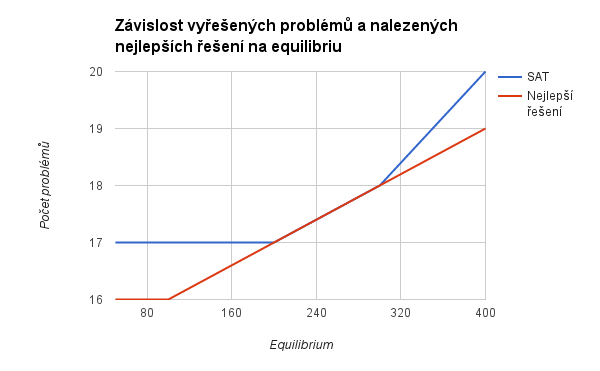
\includegraphics[width=0.99\textwidth]{6}
\end{figure}

\begin{figure}[H]\centering
 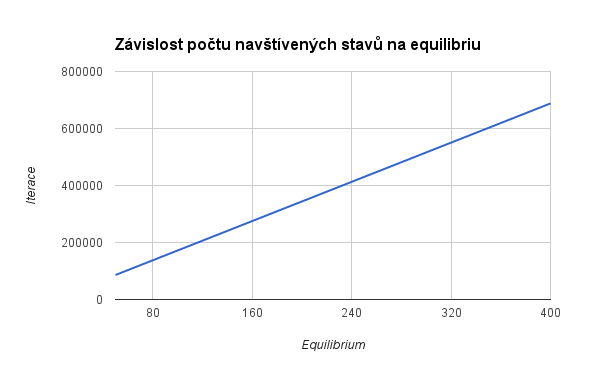
\includegraphics[width=0.99\textwidth]{7}
\end{figure}

Z grafů je možné vidět, že počet iterací je lineárně závislí equilibriu. Proto je jako ideální nastavení je zvolena hodnota 400.

\begin{table}[H]
\centering
  \begin{tabular}{ |l|l|l|l|}
  \hline
  Teplota tuhnutí & \# nalezených řešení & \# nejlepších řešení & Iterace\\
  \hline
    10  & 18 & 16 & 216000 \\
    5   & 18 & 17 & 256000 \\
    2   & 19 & 17 & 308000 \\
    1   & 19 & 17 & 344000 \\
    0,5 & 18 & 18 & 384000 \\
  \hline
  \end{tabular}
  \caption{Závislost vyřešených problémů, nalezených nejlepších řešení a iterací na teplotě tuhnutí}
\end{table}

Testované teploty tuhnutí nemají příliš vysoký vliv na výsledky algoritmu, zatímco závislost počtu iterací je spíše exponenciální. Ideální hodnota by měla být tedy minimálně 2.

\begin{figure}[H]\centering
 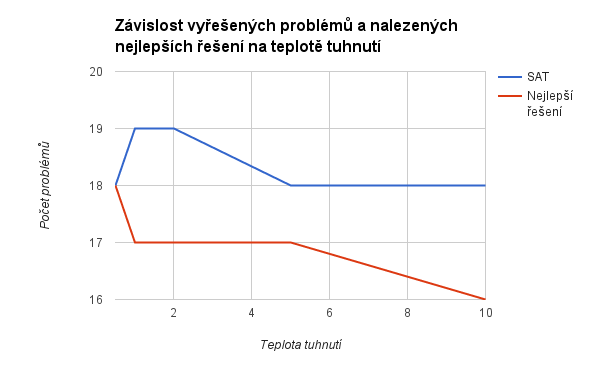
\includegraphics[width=0.99\textwidth]{8}
\end{figure}

\begin{figure}[H]\centering
 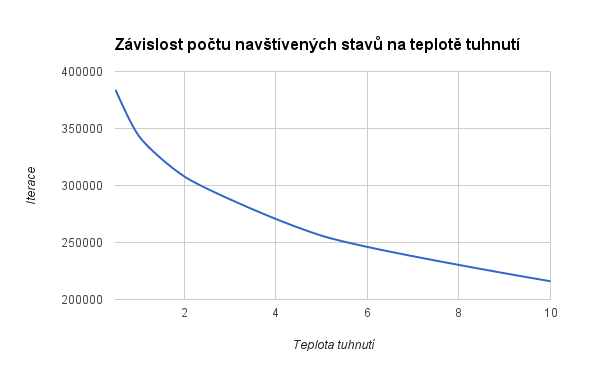
\includegraphics[width=0.99\textwidth]{9}
\end{figure}

\begin{figure}[H]\centering
 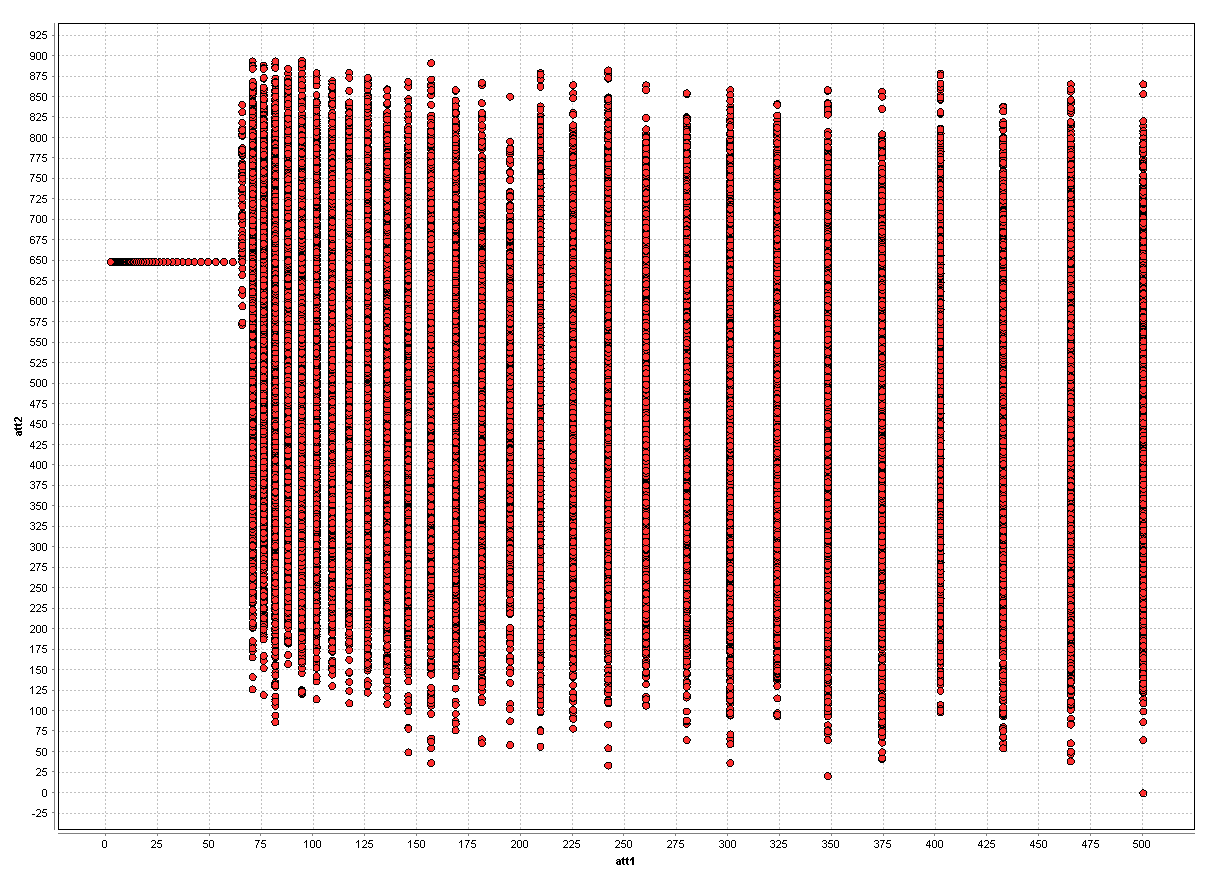
\includegraphics[width=0.99\textwidth]{weight_development}
\end{figure}

Tento graf nám zobrazuje vývoj váhy stavu v závislosti na teplotě. Pro výpočet tohoto problému byly zvoleny parametry počáteční teplota 500, koeficient ochlazování 0,93, koncová teplota 2 a $equilibrium$ 400.

Na grafu je vidět ustálení na nejlepším řešení \uv{SAT} při klesání k teplotě tuhnutí. I přesto, že jsou nalezeny stavy, které mají lepší váhu. Tato vlastnost je způsobena nastavením koeficientu zvýhodnění.

\subsection{Obtížnost SAT problémů}
Tento graf nám zobrazuje závislost obtížnosti SAT problémů na poměru klauzulí k proměnným a počtu proměnných. Byl prezentován v \emph{Stochastic Search And
Phase Transitions: AI Meets Physics} od Barta Selmana. Nejtěžší problémy jsou tedy u poměru 4,3.
\begin{figure}[H]\centering
 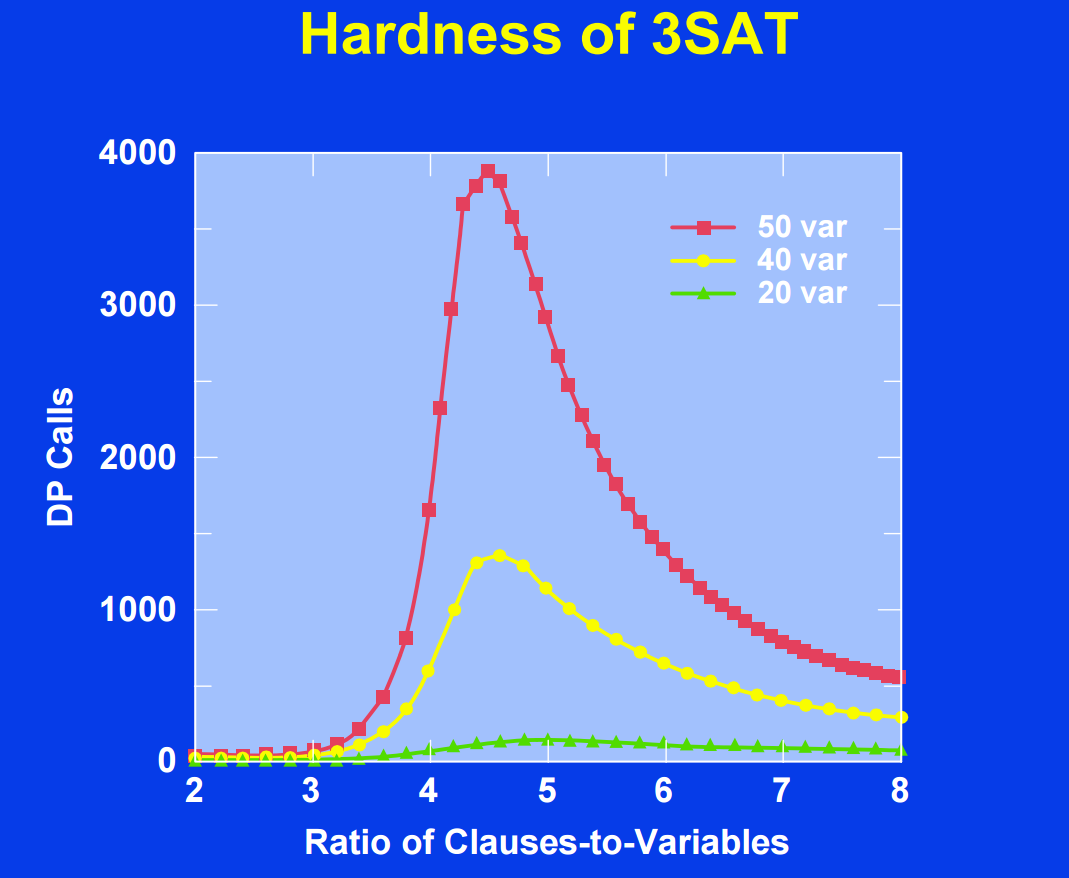
\includegraphics[width=0.99\textwidth]{sat_hardness}
 \label{hardness}
\end{figure}

\section{Závěr} 
Z naměřených hodnot je možné odhadnout vhodné nastavení implementovaného programu na: počáteční teplota 500, koeficient ochlazování 0,93, koncová teplota 2 a $equilibrium$ 400. Toto je ovšem nastavení pro instance 20 proměnných a 91 klauzulí (poměr 4,55). 

Pro těžší problémy (podle grafu \uv{Hardness of 3SAT}) např. 50 proměnných a 218 klauzulí (poměr 4,36), výše zmíněné nastavení není ideální, pro nalezení řešení je nutné více iterací algoritmu.

Dle naměřených hodnot je možné usuzovat vhodné zvyšování equilibria, které má lineární závislost k počtu iterací, a počáteční teploty. Ostatní parametry by měly být ideálně na svých hodnotách zafixovány, protože buď při zvyšování dochází k příliš prudkému počtu iterací (koeficient ochlazování) nebo u teploty tuhnutí její zmenšování příliš neovlivňuje výsledky.

Z naměřených výsledků bych metodu simulovaného ochlazování neoznačil za příliš vhodnou pro tento typ problému. Vhodné nastavení by bylo nutné najít pro každý typ instance zvlášť.

\end{document}